% The key schedule of SPARX-128/128

\begin{minipage}{0.45\textwidth}
    \begin{center}
        \captionsetup{type=figure}
        \captionsetup{width=.9\linewidth}
        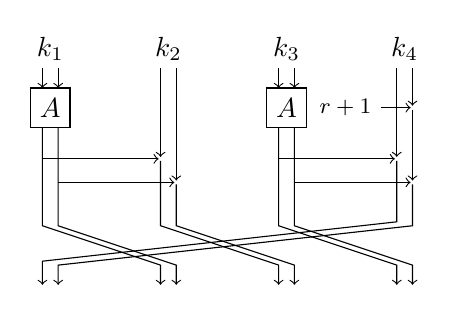
\begin{tikzpicture}[scale=0.5]
            %% input
            \draw (-4.5, +5.0) node(x0){$k_1$} ;
            \draw (-1.5, +5.0) node(x1){$k_2$} ;
            \draw (+1.5, +5.0) node(x2){$k_3$} ;
            \draw (+4.5, +5.0) node(x3){$k_4$} ;
            \draw[->] (-4.7, +4.5) -- (-4.7, +4.0) ;
            \draw[->] (-4.3, +4.5) -- (-4.3, +4.0) ;
            \draw[->] (+1.3, +4.5) -- (+1.3, +4.0) ;
            \draw[->] (+1.7, +4.5) -- (+1.7, +4.0) ;
            %% S-Box layer
            \draw (-5.0, +3.0) rectangle node[pos=0.5]{$A$} (-4.0, +4.0) ;
            \draw (+1.0, +3.0) rectangle node[pos=0.5]{$A$} (+2.0, +4.0) ;
            %% additions
            \draw (-1.7, +2.2) node[inner sep=0](add0){$\boxplus$} ;
            \draw (-1.3, +1.6) node[inner sep=0](add1){$\boxplus$} ;
            \draw[->] (-4.7, +2.2) -- (add0) ;
            \draw[->] (-4.3, +1.6) -- (add1) ;
            \draw (+4.3, +2.2) node[inner sep=0](add2){$\boxplus$} ;
            \draw (+4.7, +1.6) node[inner sep=0](add3){$\boxplus$} ;
            \draw[->] (+1.3, +2.2) -- (add2) ;
            \draw[->] (+1.7, +1.6) -- (add3) ;
            \draw (+4.7, +3.5) node[inner sep=0](addC){$\boxplus$} ;
            \draw (+3.0, +3.5) node(C){\footnotesize $r+1$} ;
            \draw[->] (C) -- (addC) ;
            % Data path
            \draw[->] (-4.7, 3.0) -- (-4.7, 0.5) -- (-1.7, -0.5) -- (-1.7, -1.0) ;
            \draw[->] (-4.3, 3.0) -- (-4.3, 0.5) -- (-1.3, -0.5) -- (-1.3, -1.0) ;
            \draw[->] (+1.3, 3.0) -- (+1.3, 0.5) -- (+4.3, -0.5) -- (+4.3, -1.0) ;
            \draw[->] (+1.7, 3.0) -- (+1.7, 0.5) -- (+4.7, -0.5) -- (+4.7, -1.0) ;
            \draw[->] (-1.7, 4.5) -- (add0);
            \draw[->] (add0) -- (-1.7, 0.5) -- (+1.3, -0.5) -- (+1.3, -1.0) ;
            \draw[->] (-1.3, 4.5) -- (add1) ;
            \draw[->] (add1) -- (-1.3, 0.5) -- (+1.7, -0.5) -- (+1.7, -1.0) ;
            \draw[->] (+4.3, 4.5) -- (add2) ;
            \draw[->] (add2) -- (+4.3, 0.6) -- (-4.7, -0.4) -- (-4.7, -1.0) ;
            \draw[->] (+4.7, 4.5) -- (addC) ;
            \draw[->] (addC) -- (add3) ;
            \draw[->] (add3) -- (+4.7, 0.5) -- (-4.3, -0.5) -- (-4.3, -1.0) ;
        \end{tikzpicture}
        \FigDef{sparx128ks128}{The 128-bit permutation $K_{4}^{128}$ used in \spnARXinstance{128}{128}.}
    \end{center}
\end{minipage}
\hspace{1em}
\begin{minipage}{0.5\textwidth}
    \begin{center}
        \captionsetup{type=algorithm}
        \setstretch{1.1}
        \begin{algorithmic}
            \State{$r \gets r + 1$}
            \State{$k_1 \gets A(k_1)$}
            \State{$(k_2)_L \gets (k_2)_L + (k_1)_L \mod 2^{16}$}
            \State{$(k_2)_R \gets (k_2)_R + (k_1)_R \mod 2^{16}$}
            \State{$k_3 \gets A(3_2)$}
            \State{$(k_4)_L \gets (k_4)_L + (k_3)_L \mod 2^{16}$}
            \State{$(k_4)_R \gets (k_4)_R + (k_3)_R + r \mod 2^{16}$}
            \State{$k_1, k_2, k_3, k_4 \gets k_4, k_1, k_2, k_3$}
        \end{algorithmic}
        \AlgDef{sparx128ks128}{Pseudo-code of $K_{4}^{128}$.}
    \end{center}
\end{minipage}